% Geometic Sum, Basic

\begin{exposition}\index{geometric sum}
Let's look at what happens if we sum powers of two.
\begin{align*}
    S_n&=\sum_{i=0}^n 2^i=1+2+4+8+\cdots+2^n\\[20pt]
    S_n&=\sum_{i=0}^3 2^i=
\end{align*}

\begin{figure}[H]
    \centering
    % \inputtikz{powersoftwosum}
    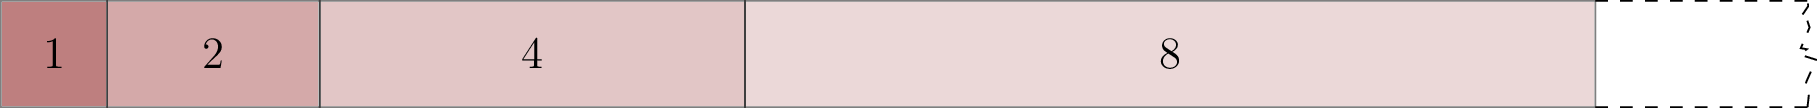
\includegraphics[alt={Visual representation of adding powers of two},width=0.85\linewidth]{images/created/powersoftwosum.png}
    \caption{Summing Powers of Two}
    \label{fig:powersoftwo}
\end{figure}

For \(n=10\):
\begin{align*}
    S_{10}&=1+2+4+8+\cdots+2^9+2^{10}\\
    2\cdot S_{10}&=2+4+8+16+\cdots+2^{10}+2^{11}\\[30pt]
    2\cdot S_{10}-S_{10}&= \\[30pt]
    S_{10}&=
\end{align*}\vspace{20pt}

For \(n=k\):
\begin{align*}
    S_{k}&=1+2+4+\cdots+2^{k-1}+2^k\\
    2\cdot S_{k}&=2+4+8+\cdots+2^{k}+2^{k+1}\\[30pt]
    2\cdot S_{k}-S_{k}&= \rule{3in}{0.2pt}\\[30pt]
    S_{k}&=
\end{align*}\vspace{20pt}

\end{exposition}

\clearpage

% Geometric sum Definition

\begin{defn}[Geometric Sum]\index{geometric sum}
    A \emph{geometric sum} is a summation of the form
    \[\sum_{i=0}^n a r^n\]
    which has the property that the ratio of any two consecutive terms is a constant ratio, \(r\).
\end{defn}


% Geometic Sum, Basic

\begin{practiceprob}
Now consider the sum of powers of 1/2.
    \begin{tcolorbox}[
        sidebyside,righthand width=4cm,
        colback=white,colframe=white
    ]
        \begin{align*}
            S_n&=\sum_{i=0}^n \left(\frac{1}{2}\right)^i=1+\frac{1}{2}+\frac{1}{4}+\frac{1}{8}+\cdots+\left(\frac{1}{2}\right)^n\\[30pt]
            S_4&=\sum_{i=0}^4 \left(\frac{1}{2}\right)^i=
        \end{align*}
    \tcblower
    \begin{figure}[H]
        \centering
        % \inputtikz{sumofpowersofhalf}
        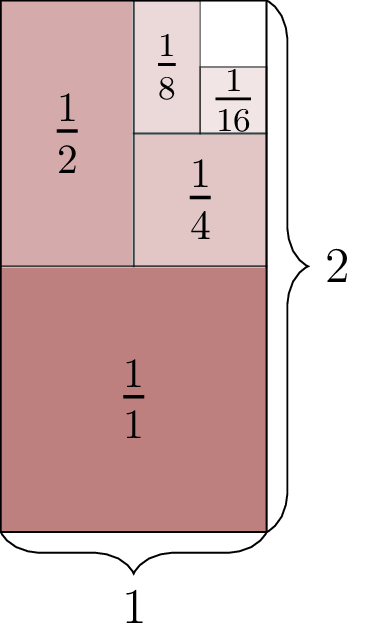
\includegraphics[alt={Visual representation of adding powers of one half},width=0.85\linewidth]{images/created/sumofpowersofhalf.png}
        \caption{Summing Powers of One Half}
        \label{fig:powerofhalfsum}
    \end{figure}
    \end{tcolorbox}

For \(n=k\):
\begin{align*}
    S_{k}&=\frac{1}{1}+\frac{1}{2}+\frac{1}{4}+\cdots+\left(\frac{1}{2}\right)^{k-1}+\left(\frac{1}{2}\right)^k\\[10pt]
    \left(\frac{1}{2}\right) S_{k}&=\frac{1}{2}+\frac{1}{4}+\frac{1}{8}+\cdots+\left(\frac{1}{2}\right)^{k}+\left(\frac{1}{2}\right)^{k+1}\\[30pt]
    \left(\frac{1}{2}\right) S_{k}-S_{k}&=\left(\frac{1}{2}-1\right)S_{k}= \\[30pt]
    S_{k}&=
\end{align*}\vspace{30pt}
\end{practiceprob}

\clearpage

\begin{practiceprob}
Next consider the sum of powers of 1/4.
    \begin{tcolorbox}[
        sidebyside,righthand width=4cm,
        colback=white,colframe=white
    ]
        \begin{align*}
            S_n&=\sum_{i=0}^n \left(\frac{1}{4}\right)^i=1+\frac{1}{4}+\frac{1}{16}+\frac{1}{64}+\cdots+\left(\frac{1}{4}\right)^n\\[30pt]
            S_4&=\sum_{i=0}^4 \left(\frac{1}{4}\right)^i=
        \end{align*}
    \tcblower
        \begin{figure}[H]
            \centering
            % \inputtikz{sumofpowersofonequarter}
            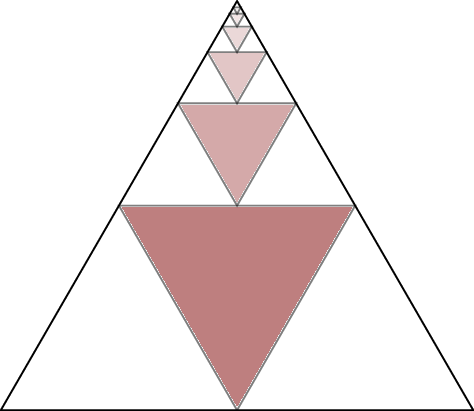
\includegraphics[alt={Visual representation of adding powers of one quarter},width=0.85\linewidth]{images/created/sumofpowersofonequarter.png}
            \caption{Summing Powers of One Quarter}
            \label{fig:sumofonequarters}
        \end{figure}
    \end{tcolorbox}

For \(n=k\):
\begin{align*}
    S_{k}&=\frac{1}{1}+\frac{1}{4}+\frac{1}{16}+\cdots+\left(\frac{1}{4}\right)^{k-1}+\left(\frac{1}{4}\right)^k\\[10pt]
    \left(\frac{1}{4}\right) S_{k}&=\frac{1}{4}+\frac{1}{16}+\frac{1}{64}+\cdots+\left(\frac{1}{4}\right)^{k}+\left(\frac{1}{4}\right)^{k+1}\\[30pt]
    \left(\frac{1}{4}\right) S_{k}-S_{k}&= \left(\frac{1}{4}-1\right)S_{k}= \\[30pt]
    S_{k}&=
\end{align*}\vspace{30pt}
\end{practiceprob}

\clearpage

\begin{exposition}[General Geometric Summation]\index{geometric sum}
Finally, what happens if we use the same strategy as before to sum multiples of powers of a common ratio.    
\begin{align*}
    S_n&=\sum_{i=0}^n a\cdot r^i=a+a\cdot r+a\cdot r^2+a\cdot r^3+\cdots+a\cdot r^n\\[40pt]
    S_4&=\sum_{i=0}^4 a\cdot r^i=
\end{align*}

For \(n=k\):
\begin{align*}
    S_{k}&=a+a\cdot r+a\cdot r^2+a\cdot r^3+\cdots+a\cdot r^n\\[10pt]
    r\cdot S_{k}&=a\cdot r+a\cdot r^2+a\cdot r^3+a\cdot r^4+\cdots+a\cdot r^{n+1}\\[40pt]
    r\cdot S_{k}-S_{k}&=\\[40pt]
    % S_{k}&=\\[40pt]
    S_{k}&=
\end{align*}\vspace{40pt}

\end{exposition}

